\documentclass[12pt]{report}
\usepackage[a4paper]{geometry}
\usepackage[myheadings]{fullpage}
\usepackage{fancyhdr}
\usepackage{lastpage}
\usepackage{graphicx, wrapfig, subcaption, setspace, booktabs}
\usepackage[T1]{fontenc}
\usepackage[font=small, labelfont=bf]{caption}
\usepackage{fourier}
\usepackage[protrusion=true, expansion=true]{microtype}
\usepackage[english]{babel}
\usepackage{sectsty}


\usepackage[UTF8]{ctex}

\usepackage{graphicx}

\usepackage{ulem}

\usepackage{xcolor}
\usepackage{listings}
\usepackage{pythonhighlight}
\usepackage{setspace}
\usepackage{indentfirst}

\usepackage{multirow}

\setlength{\parindent}{2em}


\newcommand{\HRule}[1]{\rule{\linewidth}{#1}}
\renewcommand\thesection{\arabic{section}}
\setcounter{tocdepth}{5}
\setcounter{secnumdepth}{5}



\definecolor{dkgreen}{rgb}{0,0.6,0}
\definecolor{gray}{rgb}{0.5,0.5,0.5}
\definecolor{mauve}{rgb}{0.58,0,0.82}

\lstset{ %
  language=Octave,                % the language of the code
  basicstyle=\footnotesize,           % the size of the fonts that are used for the code
  numbers=left,                   % where to put the line-numbers
  numberstyle=\tiny\color{gray},  % the style that is used for the line-numbers
  stepnumber=2,                   % the step between two line-numbers. If it's 1, each line 
                                  % will be numbered
  numbersep=5pt,                  % how far the line-numbers are from the code
  backgroundcolor=\color{white},      % choose the background color. You must add \usepackage{color}
  showspaces=false,               % show spaces adding particular underscores
  showstringspaces=false,         % underline spaces within strings
  showtabs=false,                 % show tabs within strings adding particular underscores
  frame=single,                   % adds a frame around the code
  rulecolor=\color{black},        % if not set, the frame-color may be changed on line-breaks within not-black text (e.g. commens (green here))
  tabsize=2,                      % sets default tabsize to 2 spaces
  captionpos=b,                   % sets the caption-position to bottom
  breaklines=true,                % sets automatic line breaking
  breakatwhitespace=false,        % sets if automatic breaks should only happen at whitespace
  title=\lstname,                   % show the filename of files included with \lstinputlisting;
                                  % also try caption instead of title
  keywordstyle=\color{blue},          % keyword style
  commentstyle=\color{dkgreen},       % comment style
  stringstyle=\color{mauve},         % string literal style
  escapeinside={\%*}{*)},            % if you want to add LaTeX within your code
  morekeywords={*,...}               % if you want to add more keywords to the set
}


%-------------------------------------------------------------------------------
% HEADER & FOOTER
%-------------------------------------------------------------------------------
\pagestyle{fancy}
\fancyhf{}
\setlength\headheight{15pt}
\fancyhead[L]{姓名:蓝宇霆,顾诗轩,占钰霞,王伟东,}
\fancyhead[R]{}
\fancyfoot[R]{Page \thepage\ of \pageref{LastPage}}
%-------------------------------------------------------------------------------
% TITLE PAGE
%-------------------------------------------------------------------------------

\begin{document}\large

\title{ \normalsize \textsc{}
        \\ [2.0cm]
        \HRule{0.5pt} \\
        \LARGE \textbf{\uppercase{车联网信号与系统大作业报告}}
        \HRule{2pt} \\ [0.5cm]
        \normalsize \today \vspace*{5\baselineskip}}

\date{}

\author{
        小组成员:蓝宇霆,顾诗轩,占钰霞,王伟东,马嘉琪\\
        }

\maketitle
\tableofcontents
\newpage

\sectionfont{\scshape}
%-------------------------------------------------------------------------------

%-------------------------------------------------------------------------------
% BODY
%-------------------------------------------------------------------------------

\section{基于图像增强的CNN分类和单目测距
}
\subsection{背景}
随着汽车工业的迅速发展,交通事故成为重要的社会问题。截止到了当下,交通事故已经成为了人类非正常死亡的最大直接原因之一。

而据研究显示,80\%的交通事故都源于驾驶员反应不及时,若驾驶员能够提前1秒进行操作,
则可避免90\%的事故发生。因此,防止车防追尾,控制前车距离就尤其重要。

单目测距是一种考虑单个摄像头的测距方法,但是在复杂道路的情况下,单目测距只能够反应前车的相对位置和相对距离并且因为汽车车型的类别变化,很难通过单目测距得到较为准确的前车距离。


卷积神经网络的提出(CNN),图片分类卷积神经网络是近些年逐步兴起的一种人工神经网络结构, 因为利用卷积神经网络在图像和语音识别方面能够给出更优预测结果, 这一种技术也被广泛的传播可应用. 卷积神经网络最常被应用的方面是计算机的图像识别, 它对图片上每一小块像素区域进行处理, 这种做法加强了图片信息的连续性,从而可以获得高准确度的图片识别率。

\begin{figure}[h]
  \centering
  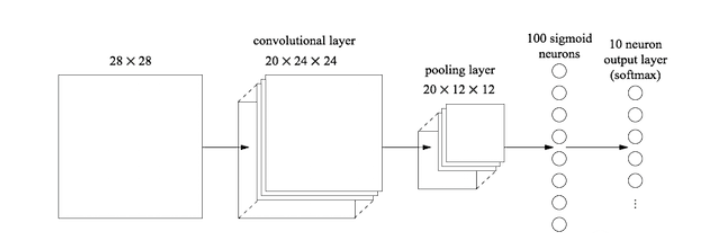
\includegraphics[width=.8\textwidth]{1.png} %1.png是图片文件的相对路径
  \caption{CNN} %caption是图片的标题
  \label{img} %此处的label相当于一个图片的专属标志,目的是方便上下文的引用
\end{figure}




通过图片增强来扩充数据,深度卷积网络自身拥有强大的表达能力,不过正因如此,网络本身需要大量甚至海量数据来驱动模型训练,否则便有极大可能陷入过拟合的窘境。可在有限的条件下,我们无法提供大量数据来训练模型。因此,在实践中数据增强便成为深度模型训练的第一步。有效的数据增强不仅能扩充训练样本数量,还能增加训练样本的多样性,一方面可避免过拟合,另一方面又会带来模型性能的提升。

\begin{figure}[h]
  \centering
  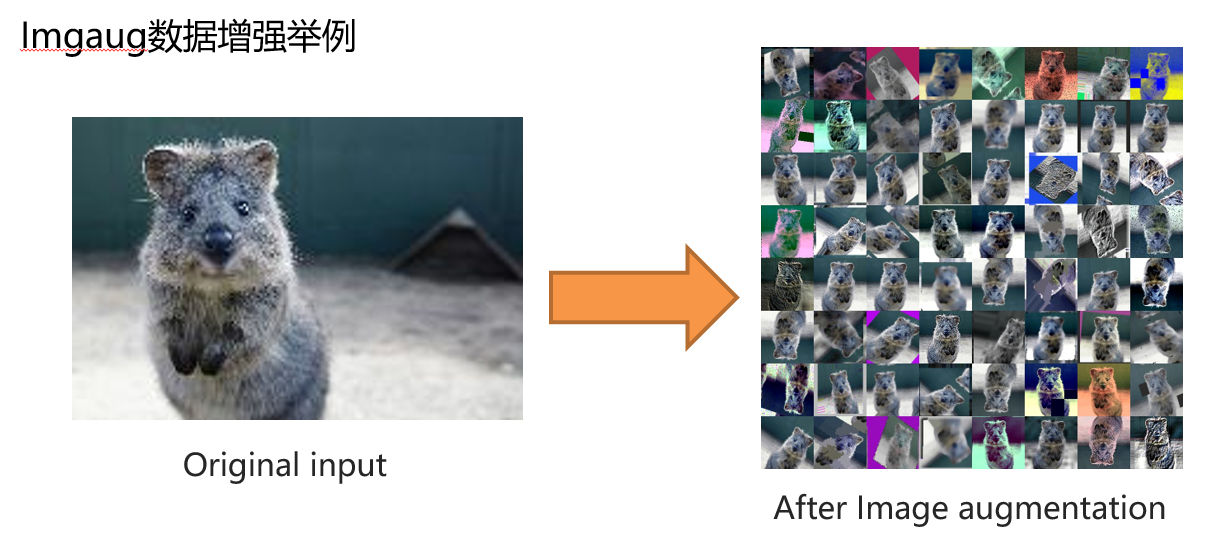
\includegraphics[width=.8\textwidth]{2.png} %1.png是图片文件的相对路径
  \caption{imgaug} %caption是图片的标题
  \label{img2} %此处的label相当于一个图片的专属标志,目的是方便上下文的引用
\end{figure}

\subsection{算法设计}
我们本次采用了基于汽车分类的前车测距,主要是基于图片增强的汽车分类和识别的基础上,根据不同种类的汽车的高度,建立一个很小的训练集(每个种类一张图片),对摄像头进行标定,求出摄像头的焦距,然后再通过这个摄像头进行单目测距。

\subsection{图片增强}
\subsubsection{简介}
图片增强的方法有很多,比如\\
1、旋转和反射变换(Rotation/reflection): 随机旋转图像一定角度; 改变图像内容的朝向;
翻转变换(flip): 沿着水平或者垂直方向翻转图像;

2、缩放变换(zoom): 按照一定的比例放大或者缩小图像;
平移变换(shift): 在图像平面上对图像以一定方式进行平移; 
可以采用随机或人为定义的方式指定平移范围和平移步长, 沿水平或竖直方向进行平移. 改变图像内容的位置;

3、尺度变换(scale): 对图像按照指定的尺度因子, 进行放大或缩小; 或者参照SIFT特征提取思想, 利用指定的尺度因子对图像滤波构造尺度空间. 改变图像内容的大小或模糊程度;

4、对比度变换(contrast): 在图像的HSV颜色空间,改变饱和度S和V亮度分量,保持色调H不变. 对每个像素的S和V分量进行指数运算(指数因子在0.25到4之间), 增加光照变化;

5、噪声扰动(noise): 对图像的每个像素RGB进行随机扰动, 常用的噪声模式是椒盐噪声和高斯噪声;

6、颜色变换(color): 在训练集像素值的RGB颜色空间进行PCA, 得到RGB空间的3个主方向向量,3个特征值, p1, p2, p3, λ1, λ2, λ3.

\subsubsection{关键代码和相关描述}
\begin{python}
seq = imgaug.augmenters.Sequential([
    imgaug.augmenters.Fliplr(0.5),
    imgaug.augmenters.Flipud(0,5),
    often(
        imgaug.augmenters.Affine(
            scale=(0.9,1.1),
            translate_percent=(0.05,0.1),
            rotate=(-10,10),
            shear=(-5,5),
            order=1,
            cval=0,
        )
    )
\end{python}
我们通过often ,rarely等函数来控制对图片处理出现的频率和次数

比如我们这里采用了Fliplr函数和Flipud函数和Affine函数.\\Fliplr主要是水平翻转/镜像输入图像.\\
\begin{figure}[h]
 
  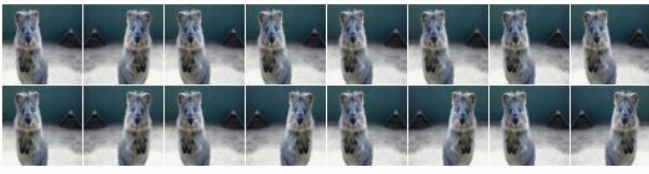
\includegraphics[width=.8\textwidth]{Floplr.png} %1.png是图片文件的相对路径
  \caption{Fliplr} %caption是图片的标题
  \label{img2} %此处的label相当于一个图片的专属标志,目的是方便上下文的引用
\end{figure}\\Flipud主要是垂直翻转/镜像输入图像.\\
\begin{figure}[h]
  
  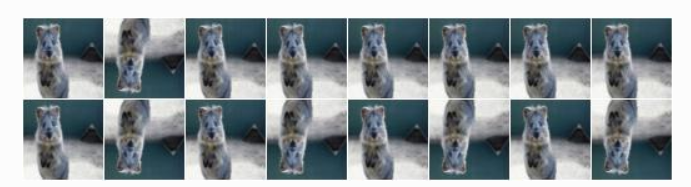
\includegraphics[width=.8\textwidth]{Flipud.png} %1.png是图片文件的相对路径
  \caption{Flipud} %caption是图片的标题
  \label{img2} %此处的label相当于一个图片的专属标志,目的是方便上下文的引用
\end{figure}\\Affine是
对图像应用仿射变换的增广器。
\\



\begin{figure}[h]
 
  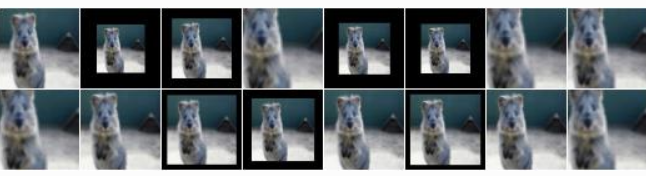
\includegraphics[width=.8\textwidth]{A.png} %1.png是图片文件的相对路径
  \caption{Affine} %caption是图片的标题
  \label{img2} %此处的label相当于一个图片的专属标志,目的是方便上下文的引用
\end{figure}

\begin{python}

    imgaug.augmenters.SomeOf((0,5),
    [
        rarely(
            imgaug.augmenters.Superpixels(
                p_replace=(0,1.0),
                n_segments=(20,200)
            )
        ),

        imgaug.augmenters.OneOf([
            imgaug.augmenters.GaussianBlur(0, 3.0),
            imgaug.augmenters.AverageBlur(k=(2,4)),
            imgaug.augmenters.MedianBlur(k=(3,5))
        ]),
\end{python}
oneof是列表增强器,它只将其部分子项应用于图像.\\Superpixels将图像完全或部分转换为超像素表示。
每个图像生成大约64个超级像素。用其平均像素颜色的50\%概率替换每一个。

\begin{figure}[h]
 
  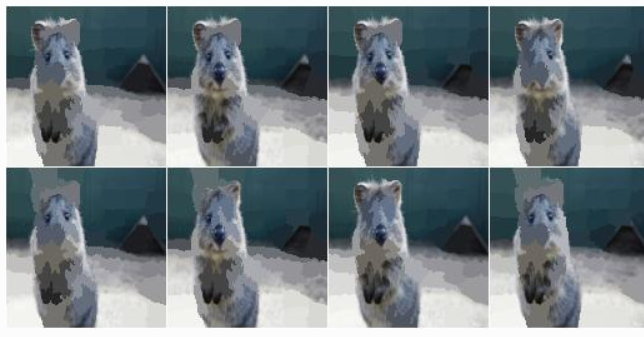
\includegraphics[width=.8\textwidth]{Super.png} %1.png是图片文件的相对路径
  \caption{Superpixels} %caption是图片的标题
  \label{img2} %此处的label相当于一个图片的专属标志,目的是方便上下文的引用
\end{figure}
\begin{python}

        imgaug.augmenters.Sharpen(alpha=(0,1.0), lightness=(0.8,1.2)),

        imgaug.augmenters.Emboss(alpha=(0,1.0), strength=(0, 2.0)),
    rarely(imgaug.augmenters.OneOf([
        imgaug.augmenters.EdgeDetect(alpha=(0,0.3)),
        imgaug.augmenters.DirectedEdgeDetect(alpha=(0,0.7), direction=(0.0,1.0)),]
    )),
        imgaug.augmenters.AdditiveGaussianNoise(
            loc=0, scale=(0.0, 0.05*255)
        ),
        
        rarely(imgaug.augmenters.Invert(0.05, per_channel=True)),

    

        imgaug.augmenters.OneOf([
            imgaug.augmenters.Multiply(mul=0.9),
            imgaug.augmenters.Multiply(mul=1.1),
        ]),

        imgaug.augmenters.Grayscale(alpha=(0.0,1.0)),

        imgaug.augmenters.ContrastNormalization((0.5,2.0)),
    ],
    random_order=True
),
    imgaug.augmenters.AddToHueAndSaturation(value=(-10,10), per_channel=True)

], random_order=True)
\end{python}

DirectedEdgeDetect增广器,检测具有特定方向的边缘并在黑白图像中标记它们,然后将结果与原始图像叠加。检测图像中具有随机方向(0到360度)的边缘,将图像转换为黑白版本,然后使用0.0到1.0之间的随机alphas将其与原始图像叠加。\par
\begin{figure}[h]


 
  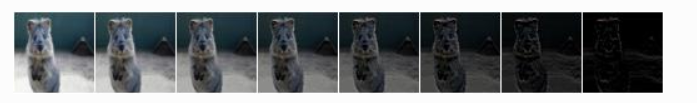
\includegraphics[width=.8\textwidth]{D.png} %1.png是图片文件的相对路径
  \caption{DirectedEdgeDetect} %caption是图片的标题
  \label{DirectedEdgeDetect} %此处的label相当于一个图片的专属标志,目的是方便上下文的引用
\end{figure}
AdditiveGaussianNoise将高斯噪声(又称白噪声)添加到图像中。
从正态分布n(0,s)中对每个像素采样一次,其中s对每个图像采样,并在0到0.05*255之间变化:

\begin{figure}[h]


 
  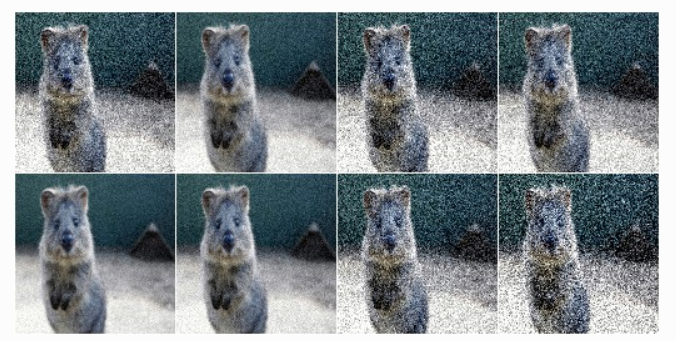
\includegraphics[width=.8\textwidth]{G.png} %1.png是图片文件的相对路径
  \caption{AdditiveGaussianNoise} %caption是图片的标题
  \label{DirectedEdgeDetect} %此处的label相当于一个图片的专属标志,目的是方便上下文的引用
\end{figure}

\subsection{基于CNN的图片分类}
\subsubsection{简介}

使用卷积神经网络(CNN)的方式对不同类型的汽车图片进行分类。使用TensorFlow实现这一操作。

首先读入图像。使用Python中的PIL库可以很容易将图像转为用于学习的矩阵数据。

定义卷积神经网络的各层级关系。卷积神经网络的组成包括输入层、卷积层、激活函数、池化层、全连接层以及输出层。

\subsubsection{代码和相关解释}
首先定义神经网络的输入层,用于存放图像数据以及其标签(即车的种类)。
\begin{python}
datas_placeholder = tf.placeholder(tf.float32, [None, 32, 32, 3])
labels_placeholder = tf.placeholder(tf.int32, [None])
\end{python}

定义神经网络的卷积层。卷积层的功能是对输入数据进行特征提取。其内部包含多个卷积核,组成卷积核的每个元素都对应一个权重系数和一个偏差量。卷积层内每个神经元都与前一层中位置接近的区域的多个神经元相连,区域的大小取决于卷积核的大小,卷积核在工作时,会有规律地扫过输入特征。在本次训练中,我们定义四层不同的卷积层,每一层使用不同数量和大小的卷积核来达到更好的效果。多次卷积可以得到图像多层次的特征,较高层次特征即是对原始特征进一步的浓缩,使得最终得到的特征更为可靠。
\begin{python}
conv0 = tf.layers.conv2d(datas_placeholder, 20, 5, activation=tf.nn.relu)
conv1 = tf.layers.conv2d(pool0, 40, 4, activation=tf.nn.relu)
conv2 = tf.layers.conv2d(pool0, 60, 3, activation=tf.nn.relu)
conv3 = tf.layers.conv2d(pool0, 80, 3, activation=tf.nn.sigmoid)
\end{python}
\begin{figure}[h]
\centering
  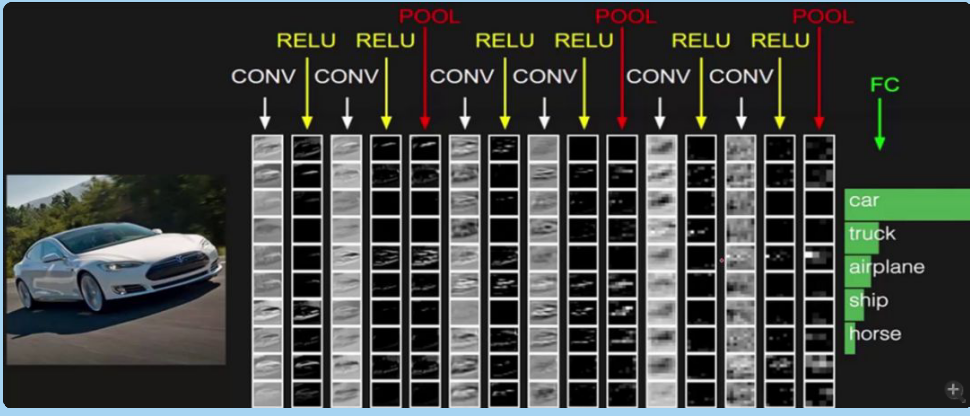
\includegraphics[width=15cm]{4.png} %1.png是图片文件的相对路径
  \caption{pic} %caption是图片的标题
  \label{DirectedEdgeDetect} %此处的label相当于一个图片的专属标志,目的是方便上下文的引用
\end{figure}

定义神经网络的池化层。池化就是对特征图进行特征压缩。在卷积层进行特征提取后,输出的特征图会被传递至池化层进行特征选择和信息过滤。池化层包含预设定的池化函数,其功能是将特征图中单个点的结果替换为其相邻区域的特征图统计量。为每一层卷积层定义其对应的池化层。
\begin{python}
pool0 = tf.layers.max_pooling2d(conv0, [2, 2], [2, 2])
pool1 = tf.layers.max_pooling2d(conv1, [2, 2], [2, 2])
pool2 = tf.layers.max_pooling2d(conv2, [2, 2], [2, 2])
pool3 = tf.layers.max_pooling2d(conv3, [2, 2], [2, 2])
\end{python}
\begin{figure}[h]
\centering
  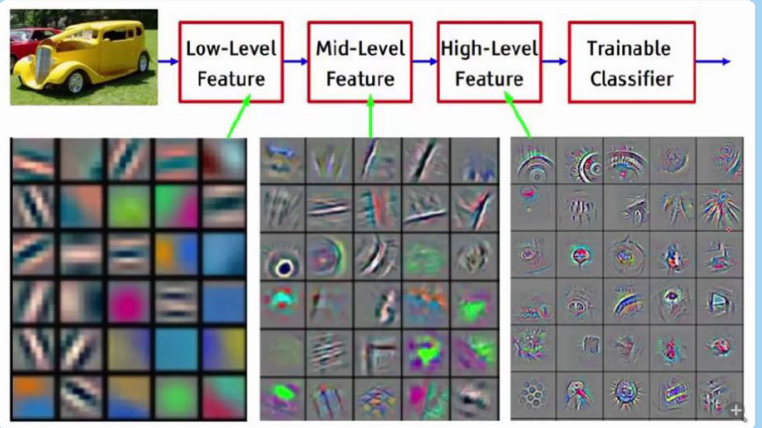
\includegraphics[width=15cm]{5.png} %1.png是图片文件的相对路径
  \caption{pic2} %caption是图片的标题
  \label{DirectedEdgeDetect} %此处的label相当于一个图片的专属标志,目的是方便上下文的引用
\end{figure}
定义神经网络的全连接层。全连接层在整个卷积神经网络中起到“分类器”的作用。卷积神经网络中的全连接层等价于传统前馈神经网络中的隐含层。全连接层通常搭建在卷积神经网络隐含层的最后部分,并只向其它全连接层传递信号。特征图在全连接层中会失去3维结构,被展开为向量并通过激励函数传递至下一层。
\begin{python}
flatten = tf.layers.flatten(pool2)
fc = tf.layers.dense(flatten, 400, activation=tf.nn.relu)
\end{python}

最后定义神经网络的输出层。对于图像分类问题,输出层使用逻辑函数或归一化指数函数输出分类标签。
\begin{python}
dropout_fc = tf.layers.dropout(fc, dropout_placeholdr)
logits = tf.layers.dense(dropout_fc, num_classes)
predicted_labels = tf.arg_max(logits, 1)
\end{python}

最后定义优化器与损失函数。利用交叉熵定义损失函数。
\begin{python}
losses = tf.nn.softmax_cross_entropy_with_logits(
    labels=tf.one_hot(labels_placeholder, num_classes),
    logits=logits
)
mean_loss = tf.reduce_mean(losses)
optimizer = tf.train.AdamOptimizer(learning_rate=1e-2).minimize(losses)
\end{python}

建立好卷积神经网络的结构后,即可开始训练。根据对测试集的判定来得出训练效果的好坏,并重新进行训练,直到一定的训练次数或者梯度下降出现收敛停止训练,得到最终的分类器。该分类器可对汽车的种类进行识别。



\begin{figure}[h]
  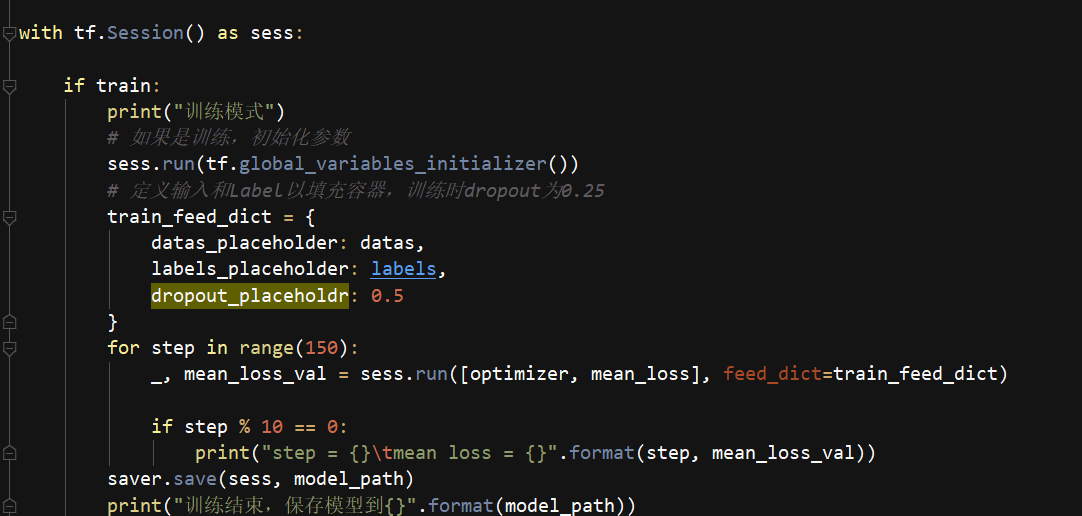
\includegraphics[width=15cm]{3.png} %1.png是图片文件的相对路径
  \caption{Traincode} %caption是图片的标题
  \label{DirectedEdgeDetect} %此处的label相当于一个图片的专属标志,目的是方便上下文的引用
\end{figure}

在测试的时候我们load 训练好的模型,然后用测试集进行测试,测试发现我们把随机识别的正确率从百分之10提升到了百分之60.
\begin{figure}
  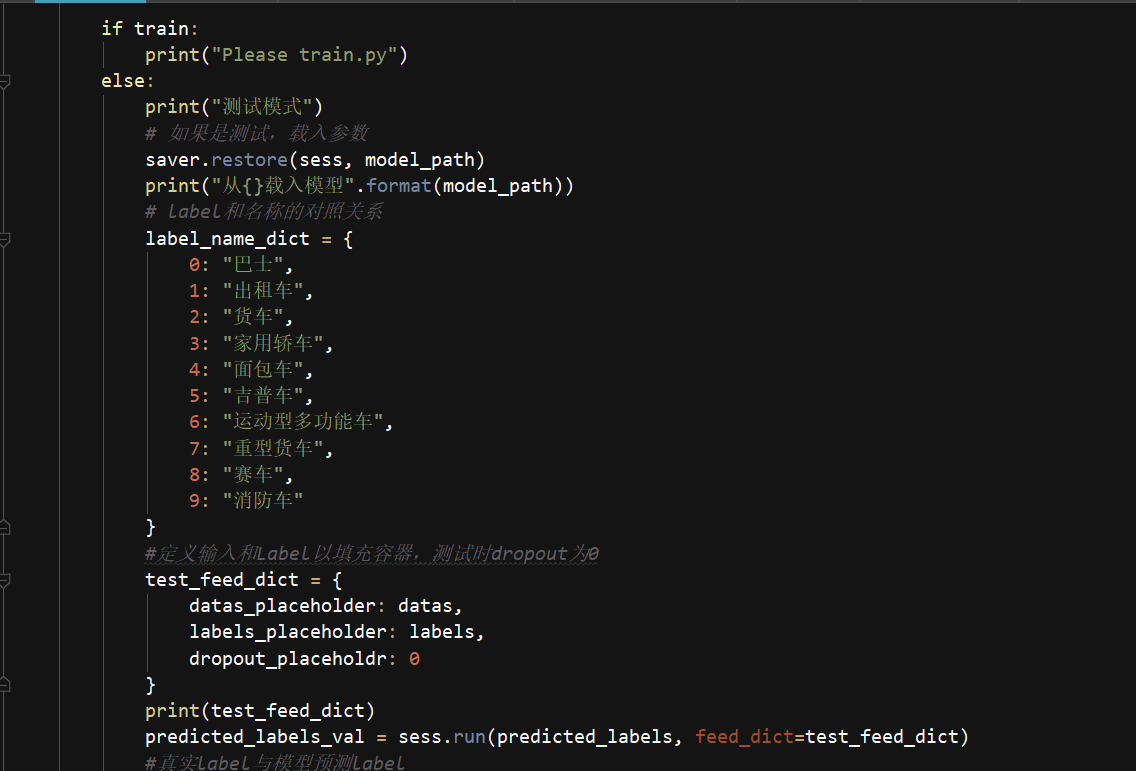
\includegraphics[width=15cm]{7.png} %1.png是图片文件的相对路径
  \caption{Testcode} %caption是图片的标题
  \label{DirectedEdgeDetect} %此处的label相当于一个图片的专属标志,目的是方便上下文的引用
\end{figure}
\subsection{单目测距}
根据摄像机的成像原理,利用相似三角形计算物体到相机的距离。
\subsubsection{简介}
由于摄像机成像本身即为一个相似变换的过程,因此,根据成像大小、像到透镜的距离、以及物体的实际大小,就能计算出物体到相机的实际距离,示意图如下:

\begin{figure}[h]

  \center
  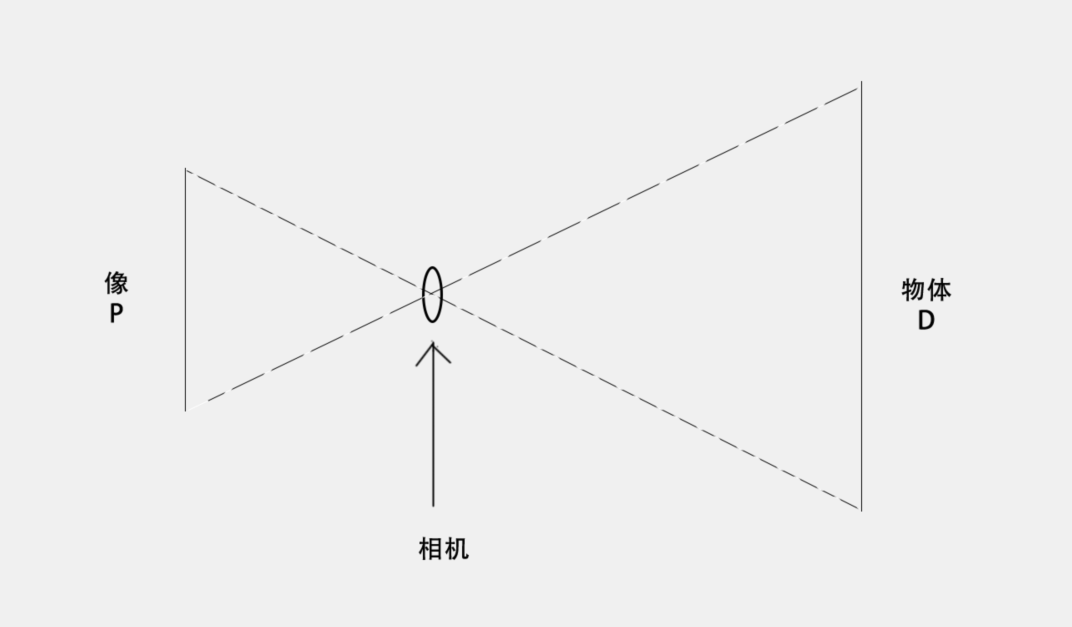
\includegraphics[width=.8\textwidth]{distance.png} %1.png是图片文件的相对路径
  \caption{figure} %caption是图片的标题
  \label{Distance} %此处的label相当于一个图片的专属标志,目的是方便上下文的引用
\end{figure}

该示意图为的摄像机成像过程,从图中可以看到,焦距、物距以及像和物体的宽度存在

\begin{equation}
F=(P*D)/W
\end{equation}
的关系

于是,由于实验采用摄像头为定焦摄像头,在定标的前提下,我们预先可以得出摄像头的焦距长度。

再根据分类器结果,得到车辆的实际宽度信息,从而计算出前方车辆到摄像头的实际距离。
\subsubsection{关键代码和相关解释}
\begin{python}
def find_marker(image):
    # convert the image to grayscale, blur it, and detect edges
    gray = cv2.cvtColor(image, cv2.COLOR_BGR2GRAY)  
    gray = cv2.GaussianBlur(gray, (5, 5), 0)        
    edged = cv2.Canny(gray, 35, 125)               
 
    # find the contours in the edged image and keep the largest one;
    # we'll assume that this is our piece of paper in the image
    (cnts, _) = cv2.findContours(edged.copy(), cv2.RETR_LIST, cv2.CHAIN_APPROX_SIMPLE)
    # get the area
    c = max(cnts, key = cv2.contourArea)
 
    # compute the bounding box of the of the paper region and return it
    # cv2.minAreaRect() 
  
    return cv2.minAreaRect(c)
\end{python}
这里是物体检测,我们考虑到了汽车的尾部和尾部上的物体是一个类似矩形的物体,这里使用了高斯模糊处理灰度图片,并且使用了canny角点检测,提取除了一个四边形,在单目摄像头中,它大概率是汽车的尾部,或者汽车尾部上的物体。c代表点集,返回rect[0]是最小外接矩形中心点坐标。 rect[1][0]是width,rect[1][1]是height,rect[2]是角度


\begin{python}
def distance_to_camera(knownWidth, focalLength, perWidth):  
    # compute and return the distance from the maker to the camera
    return (knownWidth * focalLength) / perWidth            
\end{python}

这是计算距离的函数,设计的原理就是前文提到的相似三角形,在已经知道不同长度的车型宽度的情况下进行测距。

\begin{python}
def fmain(type):
# initialize the known distance from the camera to the object, which
#type 6 means the type of one car
  if type==6:
    KNOWN_DISTANCE = 48.0
    #KNOWN_DISTANCE = 610
    # initialize the known object width, which in this case, the car

    KNOWN_WIDTH = 200
    KNOWN_HEIGHT = 16.27
    #KNOWN_WIDTH = 297
    #KNOWN_HEIGHT = 210
    # initialize the list of images that we'll be using
    #IMAGE_PATHS = ["Picture1.jpg", "Picture2.jpg", "Picture3.jpg","picture4.jpg","Picture5.jpg","Picture6.jpg","Picture7.jpg"]

    IMAGE_PATHS = ["1.jpg", "2.jpg", "3.jpg"]

# load the furst image that contains an object that is KNOWN TO BE 2 feet
# from our camera, then find the paper marker in the image, and initialize
# the focal length
    image = cv2.imread(IMAGE_PATHS[0])
#image = cv2.imread('Picture1.jpg')
#cv2.imshow('first image',image)   
    marker = find_marker(image)
    focalLength = (marker[1][0] * KNOWN_DISTANCE) / KNOWN_WIDTH
#focalLength = 811.82
    print('focalLength = ',focalLength)
    camera = cv2.VideoCapture(0)
\end{python}
Type 6意味着越野车,这里是为了展示我们已经拍到的几张图片,分别是大概站在距离车1米,然后在退后1米,再退后一米拍的三张照片,把他们命名为1.jpg,2.jpg,3.jpg,分别进行测距。
\newpage
\begin{figure}[h]

  \centering
  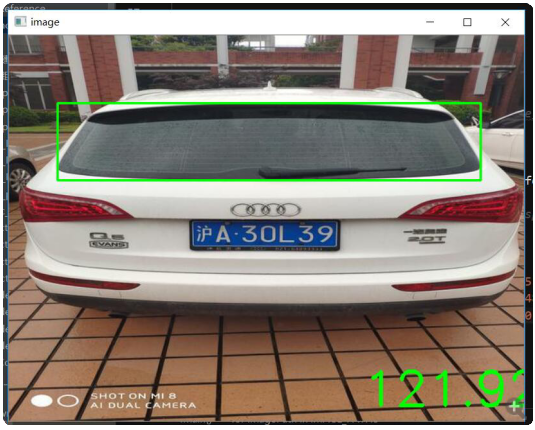
\includegraphics[scale=0.3]{11.png} %1.png是图片文件的相对路径
  \caption{1m} %caption是图片的标题
  \label{Distance} %此处的label相当于一个图片的专属标志,目的是方便上下文的引用
\end{figure}
\begin{figure}[h]
  \centering
  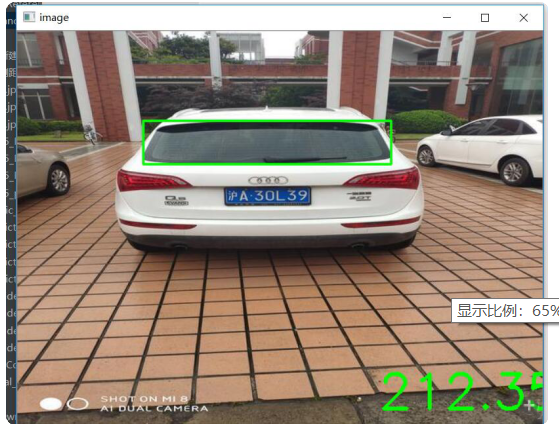
\includegraphics[scale=0.3]{12.png} %1.png是图片文件的相对路径
  \caption{2m} %caption是图片的标题
  \label{Distance} %此处的label相当于一个图片的专属标志,目的是方便上下文的引用
\end{figure}

\begin{figure}[h]
  \center
  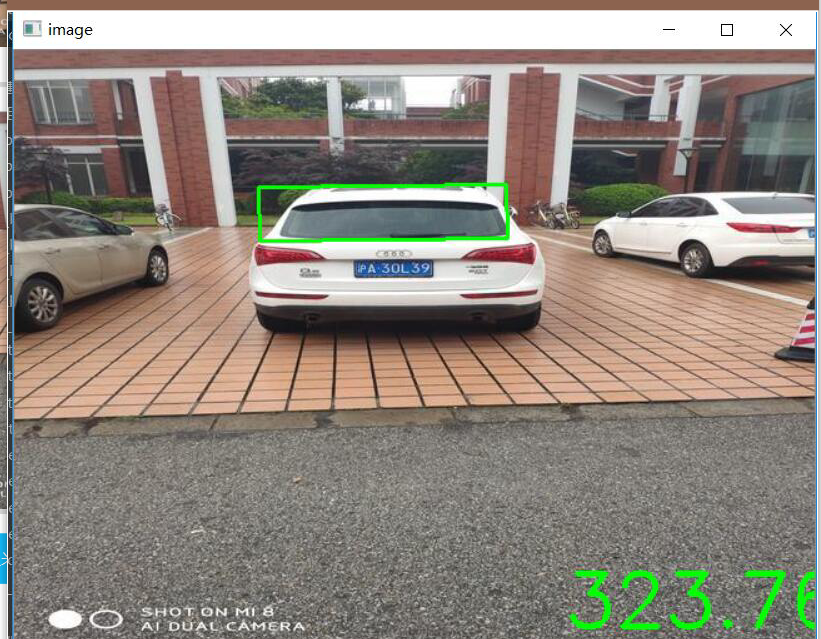
\includegraphics[scale=0.2]{13.png} %1.png是图片文件的相对路径
  \caption{3m} %caption是图片的标题
  \label{Distance} %此处的label相当于一个图片的专属标志,目的是方便上下文的引用
\end{figure}


\begin{python}
    for imagePath in IMAGE_PATHS:
    # load the image, find the marker in the image, then compute the
    # distance to the marker from the camera
        image = cv2.imread(imagePath)
        marker = find_marker(image)
        inches = distance_to_camera(KNOWN_WIDTH, focalLength, marker[1][0])

    # draw a bounding box around the image and display it
        box = cv2.boxPoints(marker)
        box = np.int0(box)
        #% (inches *30.48/ 12)
        cv2.drawContours(image, [box], -1, (0, 255, 0), 2)
        cv2.putText(image, "%.2fcm" % (inches*30.48/12),
      (image.shape[1] - 200, image.shape[0] - 20), cv2.FONT_HERSHEY_SIMPLEX,
      2.0, (0, 255, 0), 3)
        cv2.imshow("image", image)
        cv2.waitKey(0)
\end{python}

这里主要做了一个m和inch的单位换算,并且通过调用opencv的box的方法把对图片作出相应的标记。
\newpage
\section{传统方式的图像识别}
该方法是将车辆特征用相应的描述子来表示,然后用机器学习方法训练样本。
\newline\newline
目前,应用在车辆上的机器学习算法主要包括:Haar-like+Adaboost、HOG+SVM、HOG+Adaboost、HOG +Haar-like +Adaboost、阴影特征+Adaboost等方法。
\newline\newline
在基于机器视觉的车辆识别方法中,机器学习的识别方法由于具有良好的鲁棒性和优越的识别性能,使其越来越多地被应用于车辆识别当中。考虑到机器学习方法的优越性,本文使用基于Haar-like特征和Adaboost分类器的算法来对前方运动车辆进行识别。
\newline\newline
分类器的生成主要步骤为:利用类Haar特征从海量的车辆样本中提取相关特征,首先使用类Haar特征构建弱分类器,并通过Adaboost算法把弱分类器提升成为强分类器,然后把多个强分类器串联成级联分类器,得到最终的分类器。
\subsection{特征提取}
在提取Haar-like特征的部分,我们使用了积分图的计算进行操作。积分图就是只遍历一次图像就可以求出图像中所有区域像素和的快速算法,大大的提高了图像特征值计算的效率。
\newline\newline
积分图主要的思想是将图像从起点开始到各个点所形成的矩形区域像素之和作为一个数组的元素保存在内存中,当要计算某个区域的像素和时可以直接索引数组的元素,不用重新计算这个区域的像素和,从而加快了计算(这有个相应的称呼,叫做动态规划算法)。积分图能够在多种尺度下,使用相同的时间(常数时间)来计算不同的特征,因此大大提高了检测速度。
\newline\newline
大小为w×h的图像 f (x, y) 所对应的积分图像ii(a,b) 大小也为w×h 。如图所示,积分图像中每一个点 (a,b)的值是图像 f (x, y) 中从原点 (0,0) 到点(a,b) 所构成的矩形内部所有像素之和。积分图像的数学表达式如下:$$i i(a, b)=\sum_{x \leq a, y \leq b} I(x, y)$$
\newline
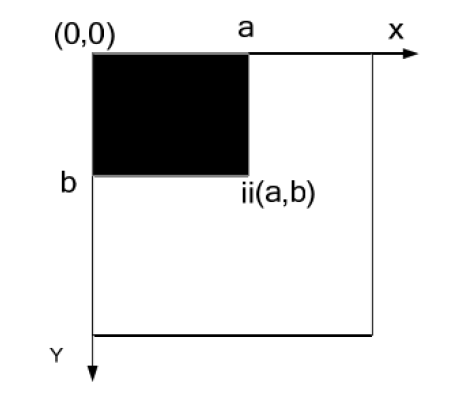
\includegraphics[scale=0.4]{ig.png}
\subsection{分类器建立}
分类器的建立首先从弱分类器开始实现,弱分类器是指分类正确率略大于50%的分类器,虽然具有结构简单、计算量小和实时性好等优点,但其分类能力较弱。本文中构建弱分类器的方法为:每一个 Haar 特征对应构建一个弱分类器。假设第 j 个 Haar 特征的特征值为 $f (x)_j$ ,则由该特征生成的弱分类器为:
$$h_{j}(x)=\left\{\begin{array}{l}{1, p_{j} f_{j}(x)<p_{j} \theta_{j}} \\ {0,other}\end{array}\right.$$
其中,$h (x)_j$ 为弱分类器的分类结果,1表示车辆目标,0表示非车辆目标;$p_j$为不等式的方向参数,取值为1或-1,1表示不等式符号为小于号,-1表示不等式符号为大于号; $\theta_j$为弱分类器$h (x)_j$的阈值。构建基于类Haar特征的弱分类器,实际上是选择一个合适的特征值作为阈值,使得该分类器对于整个训练样本集中的样本分类错误率最低。当分类器有最小分类错误率时,其对应的类Haar 特征和特征值构成最佳组合,此时的特征值就是最合适的阈值。
\newline\newline
接着用Adaboost 算法实现强分类器的构建,主要是在训练过程中动态修改各样本的权重,更多地重视其中难以识别的样本。Adaboost算法首先是进行初始化,赋予同类训练样本以相同的权重。然后才开始对训练样本进行训练,假设共需要进行T轮训练。在每一轮训练结束后,都要在降低正确分类本权重的同时,增加错误分类样本权重,从而在下次训练时更多地重视错误分类样本。在T 轮训练结束后,将获得的T 个弱分类器加权组合成强分类器,最后再用得到的强分类器。具体步骤如下:
\newline\newline
首先进行样本集准备。假设容量为 n 的样本集:$\left\{\left(x_{1}, y_{1}\right), \ldots\left(x_{i}, y_{i}\right), \ldots,\left(x_{n}, y_{n}\right)\right\}$其中,n 为样本总数;$x_i$表示第i个样本的特征向量;$y_i$表示第i个样本的标签,若是正样本记为1,负样本则记为0。假设样本集中共有l个正样本,m 个负样本,$l +m = n$,每个样本共有k个类Haar 特征。
\newline\newline
接着进行初始化权重。当 $y_i=0$ 时为负样本:$$w_{1, i}=\frac{1}{2 m}$$当 $y_i=1$ 时为正样本:$$w_{1, i}=\frac{1}{2 l}$$式中,$w_{1,i}$ 为第一轮训练中第i 个样本对应的权重。
\newline\newline
最后进行权重归一化:$$w_{t, i}=\frac{w_{t, i}}{\sum_{i=1}^{n} w_{t, i}}, i=1,2, \ldots, n$$
对于第j 个特征, 根据给定权重训练弱分类器$h_{t,j}$, ,并计算其相对于当前权重的误差$ε_{t,i}$;$$\varepsilon_{t, i}=\sum_{i=1}^{n} w_{t, i}\left|h_{t, i}\left(x_{i}\right)-y_{i}\right|$$
$$h_{t, j}=\left\{\begin{array}{l}{1, p_{j} f_{j}<p_{j} \theta_{j}} \\ {0, OTHERS }\end{array}\right.$$
$$j=1,2, \ldots k$$
式中, $h_{t,j}$ , 为弱分类器的值; $f_j$为第j 个特征的特征值; $\theta_j$为阈值;$ p_j∈{−1,1} $,表示分类方向。
\newline\newline
然后更新每个样本所对应的权重:$$\mathcal{W}_{t+1, i}=w_{t, i} \beta_{t}^{1-e_{i}}$$
式中:$\beta_{t}=\varepsilon_{t} /\left(1-\varepsilon_{t}\right)$;若样本$x_i$被正确分类,则 $e_i=0$ ;否则,$e_i=1$。
生成的强分类器如下:
$$h(x)=\left\{\begin{array}{l}{1, \sum_{t=1}^{T} \alpha_{t} h_{t}(x) \geq \frac{1}{2} \sum_{t=1}^{T} \alpha_{t}} \\ {0,Others}\end{array}\right.$$


\subsection{结果展示}
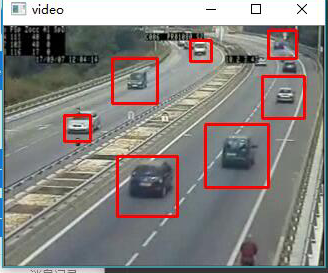
\includegraphics[scale=1]{20.png}

\section{巡线仿真}
智能车的感知部分我们完成了车尾识别与测距的实现,为了提高本项目的完整性,我们还就智能车的车辆控制部分进行了巡线仿真。
\newline\newline
具体算法设计如下:
\newline
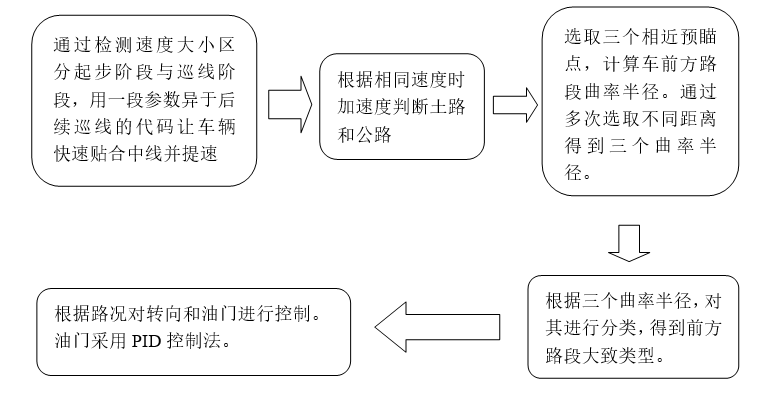
\includegraphics[scale=0.5]{cc.png}
\\代码部分在文件中已经给出,在此不做赘述。
\newline\newline
控制部分的核心算法中我们主要使用了PID,即比例积分微分控制,它是一种经典的反馈控制算法,其原理如下:
\newline 
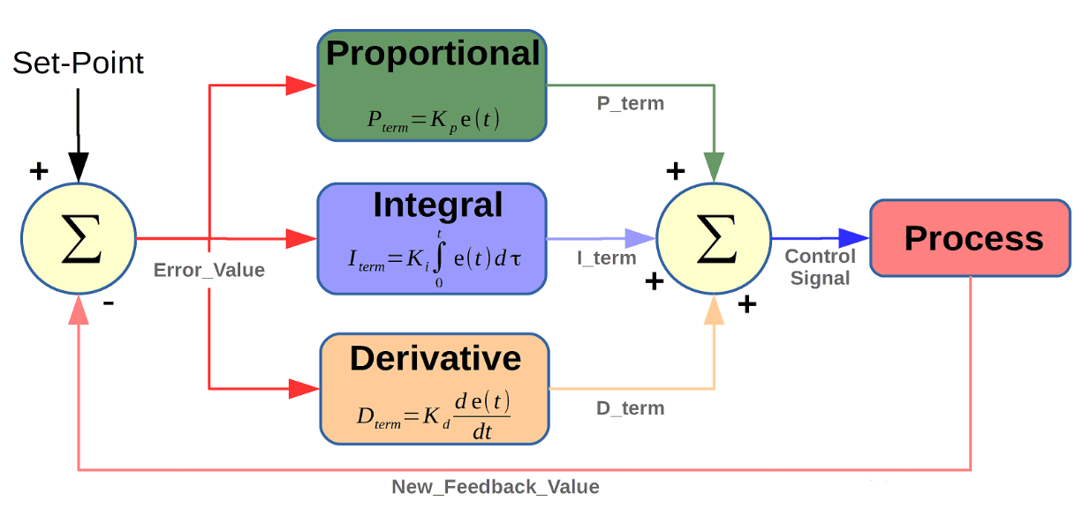
\includegraphics[scale=0.5]{pid.png}
\newline
数学表达式如下:
\newline
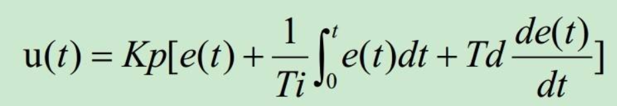
\includegraphics[scale=0.5]{PID2.png}
\newline\newline
就仿真部分而言,我们使用了CyberTORCS仿真平台进行测试,测试过程中我们使用了六种不同的路段赛道来比较,实验结果(时间单位)如下:
\newline
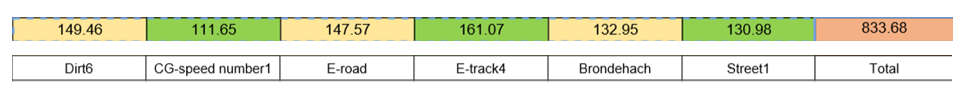
\includegraphics[scale=0.4]{res.png}
\newline\newline
仿真过程在展示中已经给出,在此给出部分截图
\newline
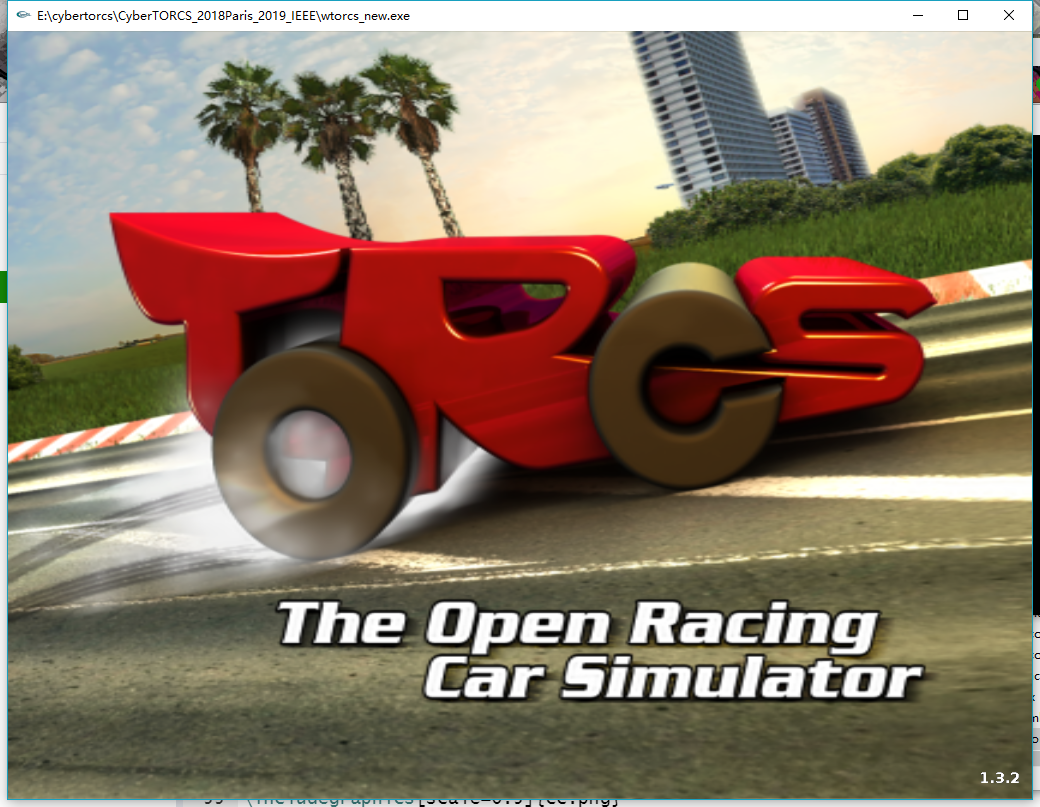
\includegraphics[scale=0.3]{t1.png}
\newline
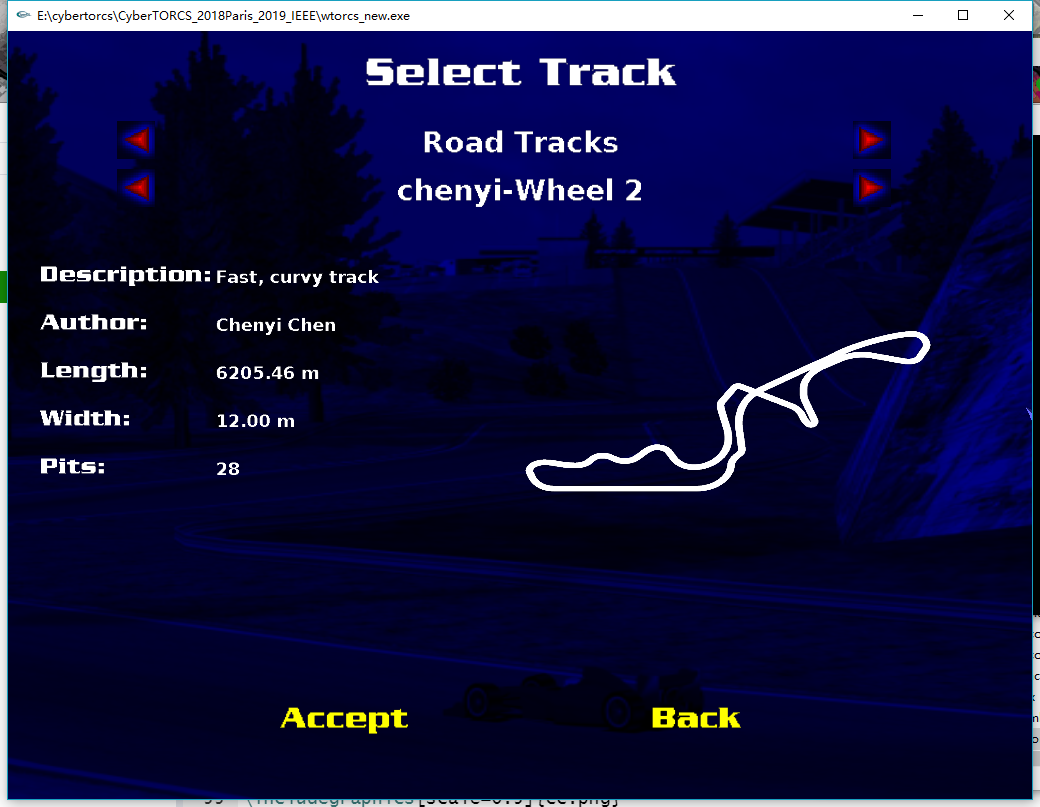
\includegraphics[scale=0.3]{t2.png}
\newline
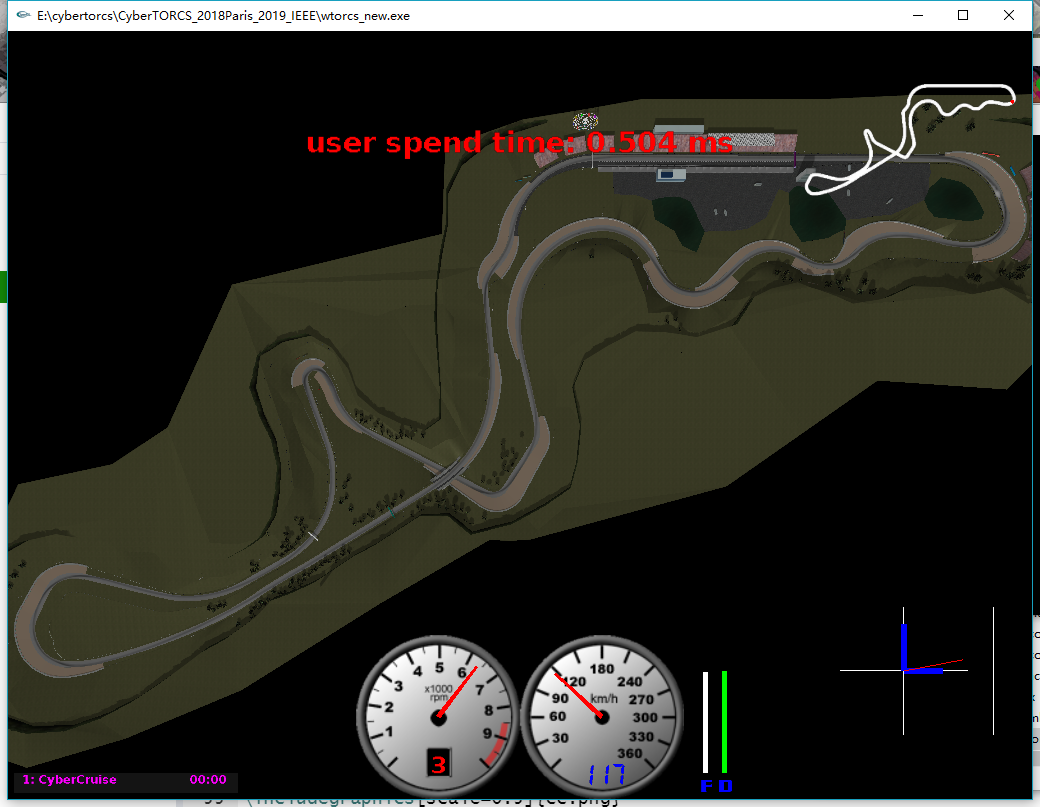
\includegraphics[scale=0.3]{t3.png}
\newline
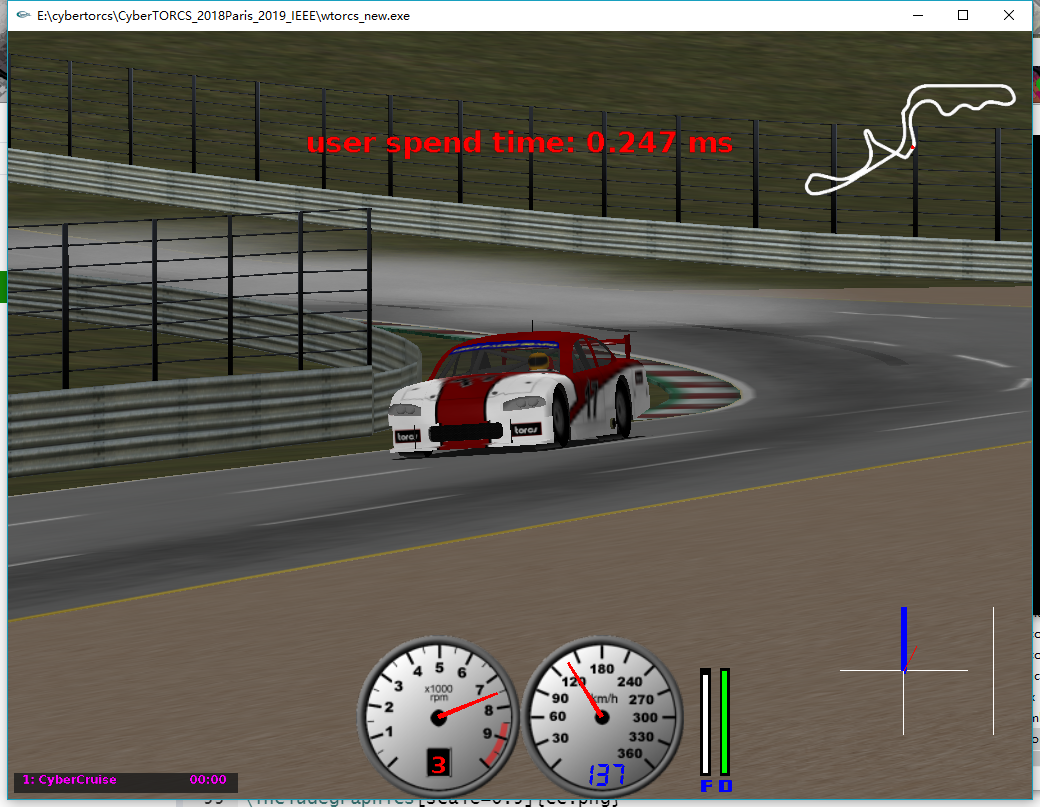
\includegraphics[scale=0.3]{t4.png}
\newline
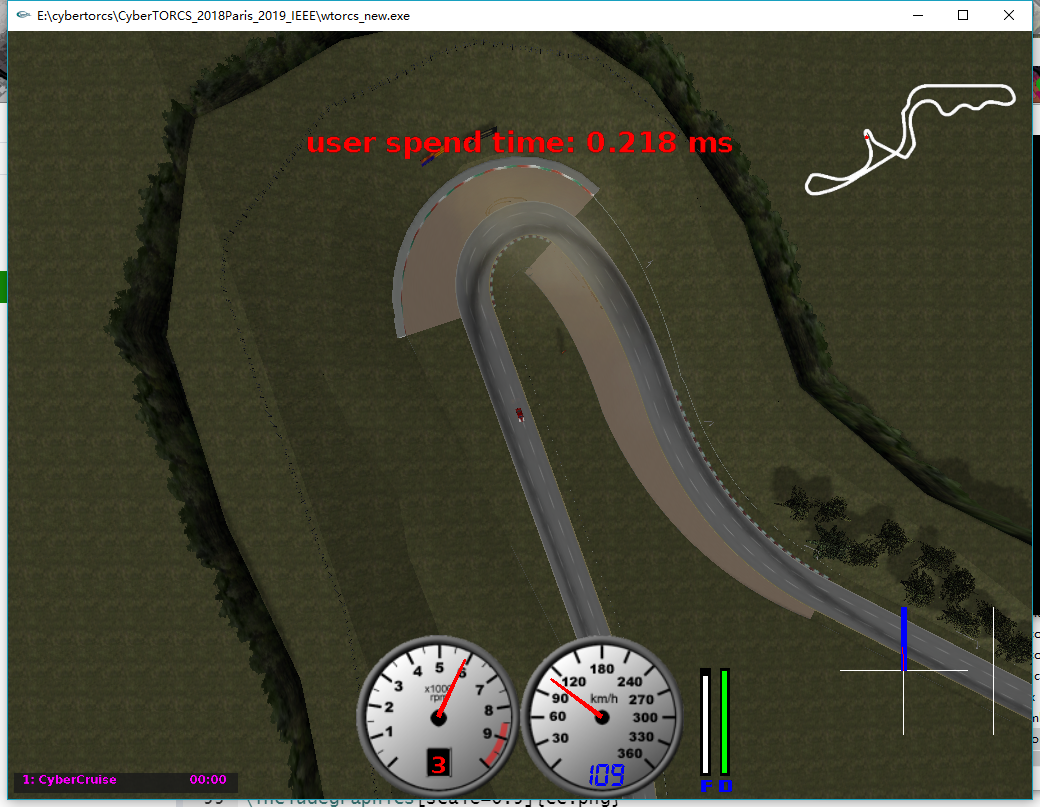
\includegraphics[scale=0.3]{t5.png}

\section{小组分工展示}
\begin{figure}[h]
  \center
  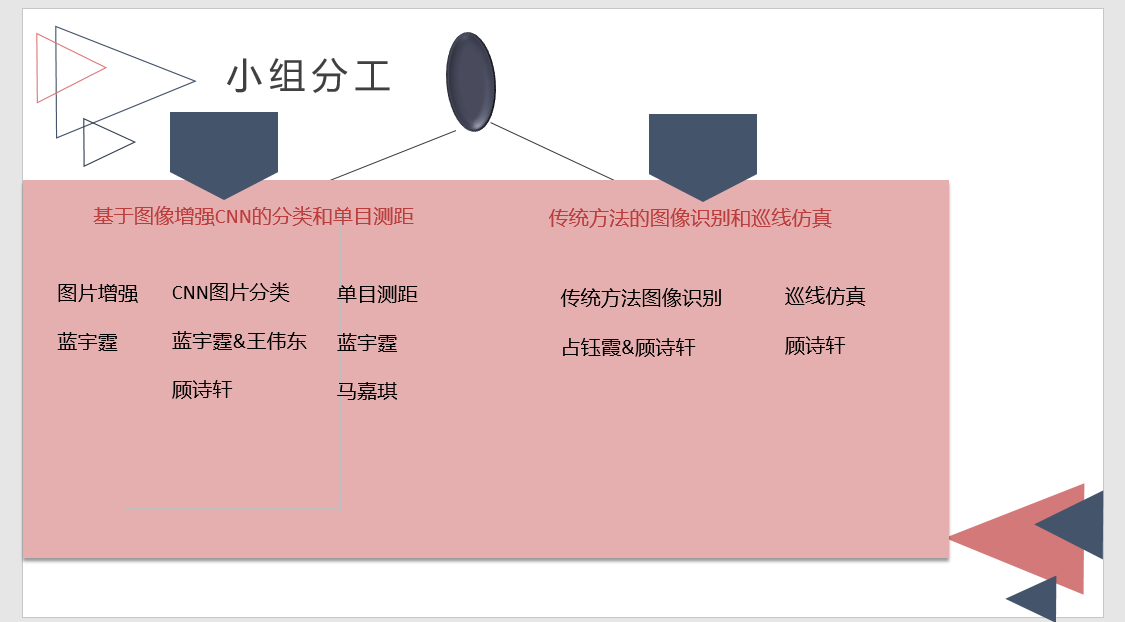
\includegraphics[scale=0.4]{re1.png} %1.png是图片文件的相对路径
  \caption{total} %caption是图片的标题
  \label{Distance} %此处的label相当于一个图片的专属标志,目的是方便上下文的引用
\end{figure}

\end{document}

